\chapter{Tecniche e Framework utilizzati}

\section{Version Control System}

Per controllare il versionamento del software durante tutta la fase di sviluppo è stato utilizzato il software \textsl{git}, in congiunzione con la piattaforma \textsl{github}:
\begin{itemize}
	\item[Maven -] https://github.com/FrancescoTerrosi/rehearsal-room-project
	\item[Gradle -] https://github.com/FrancescoTerrosi/rehearsal-room-gradle
\end{itemize}

Nonostante il lavoro sia stato svolto da un singolo studente è stato comunque adottato il modello \textsl{gitflow}, accompagnato dai meccanismi di pull-request offerti da \textsl{github}, grazie ai quali è stato possibile effettuare vari check di integrità della build su \textsl{travis}, \textsl{coveralls} e \textsl{sonarcloud}.

\section{Build Automation}

Come già detto, sono stati usati due strumenti di build automation:
\begin{itemize}
	\item Maven: solido, conosciuto e ben accettato nell'ambiente di sviluppo software, data la sua diffusione vi sono molti tutorial, plugin e schemi di configurazione
	\item Gradle: molto recente, in continuo sviluppo, permette una configurazione pressoché totale della build del progetto
\end{itemize}

\subsection{Maven}

Le specifiche di un progetto Maven vengono definite nel file "pom.xml".\newline
All'interno di questo file è possibile definire alcune opzioni di configurazione del progetto (nome del gruppo e del progetto, versione di Java\dots) e, soprattutto, definire le dipendenze necessarie al corretto funzionamento del software e i plugin che specificano le operazioni da fare durante il processo di build.\newline
Per adottare una sorta di approccio modulare anche nel processo di build del progetto, sono stati definiti diversi profili all'interno del pom.\newline
Definire un profilo permette di incapsulare i plugin e le loro configurazioni al suo interno, in modo tale che queste vengano attaccate alla fase appropriata del lifecycle di Maven solamente quando richiesto.\newline
Per separare le operazione di generazione dei report di \textsl{JaCoCo}, i \textsl{Mutation Tests}, gli \textsl{Integration Tests} e gli \textsl{End to End Tests} sono stati quindi definiti i profili:
\begin{itemize}
	\item jacoco
	\item mutation
	\item integration
	\item e2e
\end{itemize}

\begin{minipage}{\linewidth}
	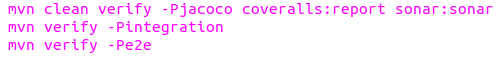
\includegraphics[width=\textwidth]{img/maven-goals.png}
	\captionof{figure}{Fasi e profili utilizzati per effettuare la build del progetto su travis-ci. Il profilo \textsl{mutation} non viene utilizzato in quanto di scarsa rilevanza per i check successivi (ma molto utile in locale)}
\end{minipage}
\newline

\subsection{Gradle}

Gradle è, attualmente, il maggior \textsl{competitor} di Maven per quanto riguarda la build automation.\newline
La procedura di assemblamento di un software è intrinsecamente diversa: se in Maven abbiamo un ciclo di vita rigido e ben definito, in cui i vari \textsl{goal} vengono eseguiti in un ordine ben definito e in maniera sequenziale, Gradle si basa sulla definizione di \textsl{tasks} (intuitivamente possiamo vederli come un corrispetivo dei \textsl{goal}), il cui ordine di esecuzione viene definito dal \textsl{task graph}, un grafo aciclico che definisce l'ordine di esecuzione dei vari compiti.\newline\newline
Il file in cui vengono definite le dipendenze del progetto, i plugin e altre configurazioni è il file "build.gradle". Uno dei vantaggi è indubbiamente l'utilizzo di un DSL \textsl{Groovy-like}, al posto del verboso xml utilizzato da Maven.\newline

\vspace{1cm}
\begin{minipage}{\linewidth}
	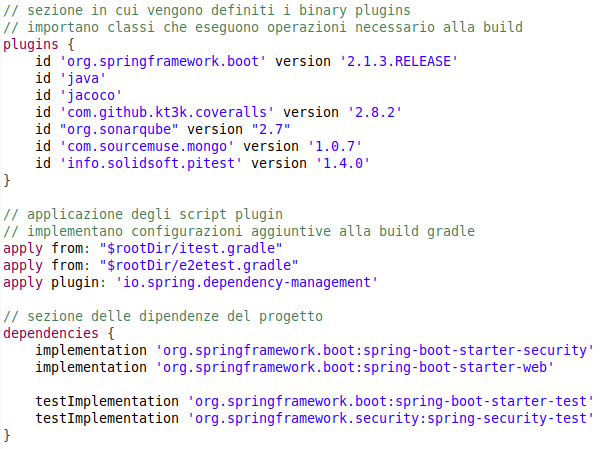
\includegraphics[width=\textwidth]{img/build-gradle.png}
	\captionof{figure}{Esempio di file build.gradle}
\end{minipage}

\pagebreak
Gradle permette inoltre di definire dei \textsl{task} personalizzati che possono essere inseriti all'interno del task graph (e quindi eseguiti ogni volta che viene eseguita la build del progetto. In questo caso possiamo immaginarli, con un certo livello di astrazione, come un \textsl{goal} di Maven che viene attaccato a una fase) oppure eseguirli in maniera autonoma.\newline\newline
Uno degli aspetti fondamentali nella definizione di nuovi task Gradle è la loro indipendenza. È buona pratica definire un file .gradle apposito in cui vengono dichiarati i \textsl{source sets} e le \textsl{dipendenze} necessarie al compimento del task, di modo tale che possa essere eseguito indipendentemente dagli altri.
È comunque possibile definire un ordinamento fra essi, utilizzando i comandi \textsl{dependsOn} e \textsl{finalizedBy}.\newline\newline
\vspace{1cm}
\begin{minipage}{\linewidth}
	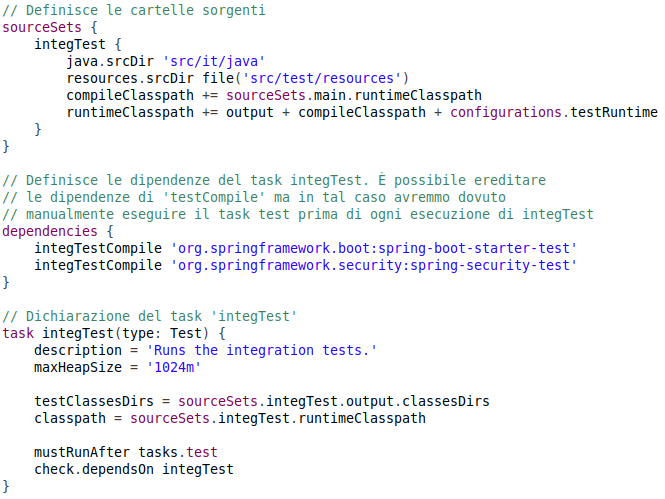
\includegraphics[width=\textwidth]{img/itest-gradle.png}
	\captionof{figure}{Esempio di task definito dall'utente nel file itest.gradle}
\end{minipage}
\newline\newline
Un altro degli aspetti fondamentali di Gradle è il massiccio utilizzo del Gradle Wrapper.\newline
Il wrapper consente di poter effettuare build gradle senza averlo installato sulla propria macchina. Lavorando in team di sviluppo il vantaggio è ancora maggiore in quanto assicura che tutti i membri effettuino le build utilizzando la stessa versione di Gradle, senza bisogno di alcuna gestione aggiuntiva.\newline\newline
Tutti i plugin e le dipendenze Maven del progetto sono state ritradotte in Gradle, per assicurare l'uniformità delle due versioni. Su travis, la build viene eseguita con il seguente comando:\newline

\begin{minipage}{\linewidth}
	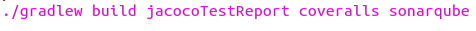
\includegraphics[width=\textwidth]{img/gradle-build.png}
	\captionof{figure}{Viene invocato il gradle wrapper per inizializzare la versione corretta di Gradle con cui eseguire la build del progetto}
\end{minipage}
\newline\newline
I task che vengono eseguiti sono:
\begin{itemize}
	\item build
	\begin{itemize}
		\item[$\rightarrow$] Configura la build e calcola il task graph, compila i file sorgente andando a scaricare le dipendenze, esegue i test e produce il fatjar dell'applicazione
	\end{itemize}
	\item jacocoTestReport
	\begin{itemize}
		\item[$\rightarrow$] Esegue JaCoCo per calcolare la code coverage
	\end{itemize}
	\item coveralls
	\begin{itemize}
		\item[$\rightarrow$] Cerca il file .xml prodotto da JaCoCo e invia i risultati a coveralls
	\end{itemize}
	\item sonarqube
	\begin{itemize}
		\item[$\rightarrow$] Effettua l'analisi su SonarCloud
	\end{itemize}
\end{itemize}
È possibile apprezzare come le operazioni per assemblare e testare effettivamente il progetto siano tutte racchiuse nel comando (task) \textsl{build}.

\section{Continuous Integration}

Per entrambi i progetti è stata stabilita un link con i server di Travis-CI, in modo tale da poter eseguire le build complete in remoto e poter continuare a lavorare localmente sul software.\newline
Le specifiche della build sono visualizzabili nel file .travis.yml, un file di configurazione che serve per dare direttive alla virtual machine su cui il progetto viene assemblato.\newline
Fra le due versioni vi è una piccola differenza: nel progetto Maven, i server MongoDB sono stati simulati attraverso l'utilizzo di Docker; per poterlo utilizzare sulla piattaforma di Travis è necessario specificarlo fra i servizi desiderati in modo tale che esso possa venire scaricato e successivamente eseguito dal plugin fabric8 in fase di testing.\newline
Nel progetto Gradle è stato invece utilizzato un plugin per avere un server MongoDB \textsl{embedded} nell'applicazione, pertanto non è stato necessario specificare l'utilizzo di Docker nel file .travis.

\section{Frameworks}

L'applicazione è stata sviluppata interamente utilizzando il framework \textsl{Spring Boot}, una delle varie soluzioni proposte dallo \textsl{Spring Framework} per la creazione di web-application in Java.\newline
L'utilizzo del framework in questione oltre ad utilizzare il meccanismo di inversione del controllo proprio di Spring, permette di sviluppare applicazioni web in maniera molto rapida, rispetto all'approccio tradizionale basato su servlet.\newline\newline
Uno degli aspetti più interessanti è appunto l'implementazione del meccanismo di \textsl{inversion of control} tramite la \textsl{dependency injection}. Dal momento che le applicazioni sviluppate con Spring Boot vengono eseguite in un web-container dove, al suo interno, viene a sua volta eseguito un server (Tomcat, in questo caso), utilizzando il meccanismo dei server embedded proprio di Spring.\newline\newline
Dal momento che risulta pressoché impossibile avere un controllo totale sull'istanziazione degli oggetti una volta che l'applicazione viene lanciata, il meccanismo di \textsl{dependency injection} è di estrema importanza. Nelle applicazioni Spring Boot, al momento del loro avvio, viene caricato un \textsl{application-context} in cui sono contenute tutte le informazioni relative ai \textsl{Bean} che non sono stati inizializzati. Attraverso l'utilizzo di questo \textsl{contesto} è possibile dunque iniettare i \textsl{Bean} nei vari oggetti al momento dell'inizializzazione dell'applicazione. Spesso è necessario definire dei file di \textsl{configurazione} per fornire informazioni aggiuntive sui Bean da creare.
\newline\newline
Un'altra importante \textsl{feature} offerta da Spring Boot sono le API per i server MongoDB. Attraverso la specifica di un semplice Bean (mongoTemplate) e la definizione dell'indirizzo IP e la porta su cui esso deve girare, è possibile connettersi al server e utilizzarlo in maniera molto intuitiva, grazie anche all'interfaccia MongoRepository.\newline
Altre feature degne di nota:
\begin{itemize}
	\item Thymeleaf: Template Engine utile per il rendering delle pagine HTML
	\item Spring-Security: Permette di implementare un meccanismo di autenticazione basato su Username e Password
	\item JUnit: framework di testing per Unit e Integration tests incorporato in Eclipse
	\item Cucumber: framework di testing per gli End-To-End tests.
\end{itemize}

\section{Software Design}

Il software implementato consiste di un Server di cui viene esposta l'interfaccia Web, accedibile tramite i consueti metodi \textsl{http} (GET, POST\dots).\newline
Inizialmente sono state definite le classi atte alla rappresentazione delle entità all'interno dell'applicazione nel pacchetto \textsl{org.unif.ft.rehearsal.model}:
\begin{itemize}
	\item BandDetails
		\begin{itemize}
			\item[$\rightarrow$] Classe che implementa l'interfaccia Spring \textsl{UserDetails}. In questa classe vengono salvate le informazioni relative a un singolo utente (che si suppone essere una band musicale). L'interfaccia \textsl{UserDetails} viene offerta da Spring come \textsl{template} per le classi che rappresentano gli utenti di un sistema.
		\end{itemize}
	\item Schedule
	\begin{itemize}
		\item[$\rightarrow$] Classe che definisce un modello per le prenotazioni. All'interno di questa classe possiamo trovare campi come: il nome della band (dell'utente) che effettua la prenotazione, data di inizio e fine, quale sala è stata prenotata\dots
	\end{itemize}
	\item RehearsalRoom
	\begin{itemize}
		\item[$\rightarrow$] Classe \textbf{ENUM} utilizzata per specificare il numero di stanze prenotabili nella sala prove.
	\end{itemize}
\end{itemize}

Gli oggetti di tipo \textsl{BandDetails} e \textsl{Schedule} possono venire salvati a runtime in un database Mongo, rispettivamente nei repository:
\begin{itemize}
	\item IBandDetailsMongoRepository
	\item IScheduleMongoRepository
\end{itemize}
La chiave primaria utilizzata è un oggetto di tipo \textsl{BigInteger} in previsione della moltitudine di record che questi possono avere.\newline\newline
A runtime tuttavia, non è possibile accedere direttamente ai metodi offerti da queste interfacce ma bisogna accedervi attraverso dei \textsl{Services}.\newline
Una classe che implementa un servizio può essere intuitivamente vista come un \textsl{wrapper} per uno specifico \textsl{repository}. Avendo a disposizione due differenti repository mongo, sono stati implementati i due seguenti servizi:
\begin{itemize}
	\item BandDetailsService
	\begin{itemize}
		\item[$\rightarrow$] Questa classe implementa uno \textsl{UserDetailsService}, implementazione necessaria per poter "immergere" questo servizio all'interno del framework Spring. Nella classe di configurazione della WebSecurity questo servizio viene specificato come \textsl{DaoAuthenticationProvider bean}, per permettere a Spring di sapere quale classe debba usare per l'autenticazione degli utenti. Questa classe utilizza un encoder BCrypt per criptare le password inserite dagli utenti.
	\end{itemize}
	\item Scheduler
	\begin{itemize}
		\item[$\rightarrow$] Classe che implementa le operazioni CRUD per gli oggetti di tipo \textsl{Schedule}
	\end{itemize}
\end{itemize}

Per mantenere traccia delle varie operazioni effettuate dai \textsl{Services}, è stata utilizzata una utility di Logging: \textsl{Logback}. Questa scelta è stata fatta perché \textsl{Logback} è l'utility predefinita di Spring.\newline
Sono stati definiti due differenti file di configurazione: uno per il logging in fase di testing (in cui i log vengono mostrati solamente su console) e uno per la fase di runtime, in cui le attività come: la registrazione di un utente, eventuali tentativi di accesso falliti (utili per rilevare tentativi di accesso illegali) e altri ancora vengono salvati in dei file di log utilizzando il protocollo di \textsl{logrotation}.\newline
Per maggiori dettagli è possibile consultare i file di configurazione:
\begin{itemize}
	\item \textsl{src/main/resources/logback.xml}
	\item \textsl{src/test/resources/logback-test.xml}
\end{itemize}

Una delle caratteristiche più interessanti di Spring è indubbiamente la possibilità di implementare feature piuttosto complesse come l'autenticazione, semplicemente andando a definire delle classi di configurazione.\newline
All'interno di questo progetto possiamo trovare due classi di questo tipo nel pacchetto \textsl{org.unifi.ft.rehearsal.configurations}:
\begin{itemize}
	\item MongoConfig
	\item WebSecurityConfig
\end{itemize}

La prima classe si occupa semplicemente di definire un \textsl{bean} MongoTemplate, un'implementazione della classe MongoOperation che implementa le principali operazioni su un mongoDB.\newline
La seconda classe di configurazione, indubbiamente più interessante, si occupa invece delle specifiche tecniche di Security per l'applicazione. Di seguito vengono riassunti gli aspetti più interessanti che possiamo trovare al suo interno:
\begin{itemize}
	\item Il metodo \textsl{configure(HttpSecurity)} è responsabile di gran parte del lavoro. Al suo interno è possibile specificare quali richieste agli URL siano ad accesso pubblico e quali invece debbano essere protetti. Inoltre è possibile specificare quale sia la pagina di Login e gli identificativi dei form in cui vengono inseriti username e password. Questo aspetto è fondamentale in quanto a questo punto Spring si occuperà in maniera autonoma delle operazioni di autenticazione (è possibile notare infatti come nella classe \textsl{LoginPageWebController} sia presente soltanto il metodo responsabile di renderizzare la pagina HTML).
	\item Il metodo \textsl{configure(WebSecurity)} si occupa invece non solo delle richieste ma del \textsl{contesto} generale dell'applicazione. In questo metodo si esclude dai controlli di security gli URI corrispondenti ai file css e alle pagine ad accesso pubblico come la \textsl{homepage} o la pagina di registrazione.
	\item La classe privata \textsl{RehearsalAuthenticationSuccessHandler} è un'implementazione dell'interfaccia \textsl{AuthenticationSuccessHandler} offerta da Spring. Viene fatto un \textsl{override} del metodo \textsl{onAuthenticationSuccess} che viene invocato ogni volta che un'autenticazione ha successo di modo tale che venga fatto il \textsl{forward} di parametri come l'username di un utente che verranno poi utilizzati come attributi di sessione, oltre che effettuare il redirect alla pagina delle prenotazioni.
\end{itemize}

Come già stato detto all'inizio di questo paragrafo, il Server espone i propri servizi attraverso un'interfaccia web: questo viene realizzato tramite i \textsl{WebController} all'interno del pacchetto \textsl{org.unifi.ft.rehearsal.web}.\newline\newline
Un Web Controller non è altro che un "mediatore" fra le operazioni fornite dalle classi di \textsl{service} e la rappresentazione grafica (html) di tali operazioni. Un Web Controller espone i servizi su degli endpoint http (e.g. /register), modifica il modello e aggiorna la vista da restituire all'utente; non a caso questo pattern viene chiamato Model View Controller ed è lo standard utilizzato da Spring.\newline
Ad eccezion fatta per \textsl{LoginPageWebController} che si occupa solo di mostrare la pagina HTML di login ed eventualmente di aggiungere un messaggio di errore nel caso di mancata autenticazione, i due controller \textsl{RegisterPageWebController} e \textsl{SchedulePageWebController} presentano un buon esempio dell'utilizzo di questo pattern. È possibile apprezzare come tramite il template-engine \textsl{Thymeleaf} si possa manipolare il codice HTML delle viste da restituire all'utente grazie a semplice codice Java e a come le richieste http degli utenti, possibilmente contenenti anche diversi parametri, vengano mappati in dei metodi che vanno ad interagire sia con le viste che con i \textsl{Services} visti in precedenza.
